\documentclass[a4paper,11pt]{article}
\usepackage{amsmath,amsfonts,amsthm,bm,listings,graphicx,float,subcaption,multicol,wrapfig,stfloats}
\usepackage[export]{adjustbox}
\usepackage[labelfont=bf]{caption}
\usepackage[margin=1.1in]{geometry}
\graphicspath{ {/Users/ianmcwilliam/Desktop/MSc/Active_Learning/Tex} }
\usepackage{titling}
\usepackage{hyperref}
\setlength{\droptitle}{0cm}

\begin{document}
\title{Informatics Project Proposal - Automatic Curriculum Learning for Deep Models Using Active Learning}
\author{Ian McWilliam s0904776}
\date{}
\maketitle


\section{Introduction}
\textit{Active learning} is a training paradigm wherein machine learning algorithms actively select, or `query', the samples from which they learn \cite{Settles 2009}; in the case of deep models this contrasts with the usual approach of uniformly sampling training instances. A related field is that of \textit{curriculum learning}, which explores how the learning process can be improved by presenting training samples to the algorithm in a meaningful order (with the order defining a `curriculum'), again in contrast to sampling uniformly from a training set \cite{Bengio 09}.

One of the main difficulties with implementing curriculum learning is deciding how to construct the curriculum\cite{Bengio 09}; in this project we will explore how active learning methods, can be used to automatically construct training curricula for deep models, enabling efficient curriculum learning without requiring extensive domain knowledge and/or building a predfined curriculum prior to training. The objective of the project is to test the hypothesis that training deep models with such `active curricula', a term we propose for curricula constructed from active learning methods, can improve upon other training paradigms such as uniform random sampling, pre-training or traditional curriculum learning. The work will investigate a variety of methodologies for constructing a curriculum using active learning metrics, focusing on how the different training methods affect the performance of convolutional networks (CNNs) on a range of image classification tasks. The output of the project will hopefully be a set of novel ways to improve the training of deep models, as well as a more thorough exploration of the relationship between active and curriculum learning than currently exists in the literature.

In the next section we will further introduce both active and curriculum learning, as well as outlining previous efforts to automate curriculum learning. We will then lay out the methods we will use in the project to construct curricula with active learning methods, before discussing how we will evaluate the methods and giving a work plan for the project.

\section{Background}
\subsection*{Active Learning}
The motivation for active learning is that by allowing the algorithm to intelligently select the samples from which it learns, it can achieve superior generalization performance, from a smaller number of training samples, than if the samples had been chosen uniformly \cite{Cohn 1994}. In domains where unlabeled data is abundant but obtaining labels is expensive, active learning can be used to reduce the cost associated with training, as the active approach allows the designer to obtain labels only for the samples which will be most beneficial to learning.

There are a variety of methods by which the algorithm can query datapoints, however they generally focus on finding the points in the input space that are most ``informative'' to the algorithm \cite{Settles 2009} allowing it to fill what could be seen as gaps in its knowledge of the domain. Methods for estimating informativeness range from approximating the algorithm's `uncertainty' in labelling a given sample, to finding which training samples have the potential to lead to the largest change in model parameters. In the case of deep models in particular, we note the work of Gal et al \cite{Gal 2016} who define uncertainty by using the uncertainty inherent in Bayesian deep models, estimated by approximating variational inference with Monte Carlo dropout methods as in \cite{Gal 2016 2}.

\subsection*{Curriculum Learning}
As mentioned in the introduction, curriculum learning focuses on improving learning by setting the order in which samples are used in training. Motivated by the way in which humans and animals learn, a curriculum generally begins with `easy' examples, before transitioning to more challenging ones, with the aim being to improve generalization performance and convergence speed. It is interesting to note that, while similar, active and curriculum learning are somewhat opposed in their learning philosophies, with the former focusing on learning from uncertain/difficult samples and the latter beginning with easy samples before continuing to more difficult ones. 

Bengio et al \cite{Bengio 09} find a theoretical motivation for curriculum learning by suggesting that it can be seen as a \textit{continuation method} (a method of optimization non-convex functions \cite{Allgower 1980}). Curriculum learning has also drawn similarities with \textit{transfer learning}, as the early, `easier' stages of training can be seen as a separate task, with the network weights then being used as the initial weights for training on more difficult samples. Similarly curriculum learning can be seen as a form of pre-training; Bengio et al \cite{Bengio 09} compare the method to unsupervised pre-training methods as in \cite{Erhan 09}, where the authors demonstrate that unsupervised pre-training allows the supervised learning to begin in a region of parameter space that results in superior generalization performance. 

One of the immediate difficulties with implementing curriculum learning is that the curriculum must be constructed prior to training, requiring some predefined measure of difficulty with which to order the training samples. In certain domains there may be a natural ordering of difficulty, for example in the geometric shapes example in \cite{Bengio 09}, however in many tasks manually constructing a curriculum is not as straight forward. This motivates the development of methods to automatically construct learning curricula without requiring expert domain knowledge; in this project we propose using active learning methods to automatically construct such curricula, potentially providing an efficient way to improve the training of deep learning algorithms. 

\subsection*{Related Work}
There have been several works that have explored the area of automating the process of constructing learning curricula, as well as similar studies which evaluate methods by which training can be improved by deviating from the usual paradigm of uniform sampling; we introduce a few of these methods here.

In the paper ``Self-Paced Learning for Latent Variable Models'', M.Pawan Kumar, B. Packar and D.Koller, 2010 \cite{Koller 2010} introduce the concept of \textit{self-paced learning}, inspired by curriculum learning. For self-paced learning, after an initial training period, a learning algorithm is trained beginning with the ``easiest'' samples, with the number of included sampling slowly increasing until the entire training set is considered. The learning algorithm explored in the paper is the latent SSVM model, and easiness in the paper is calculated from how far from the separating hyperplane a training example is. The authors test their methods on datasets from a variety of domains, specifically ``natural language processing, biology and computer vision'', illustrating that their method outperforms a baseline of training on the whole training set. The work is an interesting example of automatically constructing a curriculum but is limited to only considering the latent SSVM model, the authors also do not explore other potential curricula, for example beginning with harder examples instead of easier.

Weinshall and Cohen \cite{Weinshall 2018}, connect curriculum learning to transfer learning in a method similar to self-paced learning. They propose using a ``shallow'' learner, such an an SVM, using feature representations from a deep model pre-trained on a similar but separate task, then using the distance to margin of the SVM to select and train on the easier examples, such as in \cite{Koller 2010}. The paper is interesting as it compares curriculum learning to what they term ``anti-curriculum'' learning, i.e. training on harder examples instead of easier, as in most active learning methods. Interestingly, they conclude that, not only does the curriculum learning outperform the ant-curriculum/active learning approach, the latter fails to perform even a uniform sampling benchmark.

The paper ``Automated Curriculum Learning for Neural Networks'' by Graves et al, 2017 \cite{Graves 2017} focuses on automatically constructing curricula for neural networks, specifically deep models. The paper considers problems where learning can be split up into a series of distinct``tasks'', with the goal being either to maximise performance on all tasks, or only seeking to maximise performance on a final ``target task''. This work represents a similar goal to that of this project, automatically constructing curricula for deep models, and presents several novel approaches for selecting training samples that could be adapted for use in active learning. The use of reinforcement learning to construct the curriculum is also novel, and it is interesting to note that the final policies generally resulted in an easy to hard curriculum, with the algorithm autonomously discovering implicit orderings in task difficulty and finding that it is best to begin with easier tasks, supporting the curriculum learning rationale in \cite{Bengio 09}. The paper is limited in that it focusses on datasets where it is possible to separate different``tasks'', which is not always the case. The method also relies on having both the input features and label of all training samples, as opposed to in active learning where it is assumed the label is unknown to the learner, the method proposed in this project would function in such situations.

A similar reinforcement learning approach is found in a paper by Fan et al \cite{Fan 17}, where the authors udesign an approach called Neural Data Filtering (NDF) to adaptively select which training samples to select. As training proceeds, a reinforcement learning algorithm is used to decide which training samples should be supplied to a base model which is trained on the underlying task. As training proceeds the reinforcement algorithm updates its policy in such a way that it can adaptively select which samples will optimise learning. The paper differs from \cite{Graves 2017} in that it does not require the existence of several sub-tasks, it also compares their results to other curriculum methods such as self-paced learning, as opposed to just using a uniform baseline, something which we find few other papers do. The method is limited however in that it significantly complexifies the problem by requiring the training of a reinforcement learning algorithm alongside the training of the base model, implying significant computational cost. 

A recent paper by Chang et al, 2018 \cite{Chang 18} conducts similar experiments to the approach proposed for this project, constructing curricula by adapting the sampling probability proportionally to two metrics, specifically classification threshold proximity and prediction variance. They test their methods for training deep models on a variety of datasets, highlighting how their methods can reduce model bias in noisy environments, as illustrated in Figure 2 of \cite{Chang 18}. The authors test their training methods on a variety of datasets, including image classification and NLP tasks, showing consistent out-performance of their methods against a benchmark of uniform random sampling. The authors also explore whether or not selecting `easier' or `harder' samples lead to better results, concluding that the answer is task dependent; in easier tasks they find that it is beneficial to train on samples that the model is more uncertain about, and vice versa for more difficult, noisier problems. 

The paper is limited in that it considers a relatively limited range of uncertainty metrics and curriculum constriction methods, as well as benchmark comparisons. It would also be interesting to explore how to automatically adjust the preference for harder or easier samples throughout training in order to obtain an optimal solution, as it may be difficult to know beforehand which curriculum method will perform the best. 
\vspace{0.5cm}

While these prior works have explored methods for automatically building learning curricula, we believe the work proposed in this project presents a novel direction for several reasons. While some of the papers studied use approaches similar to those used in active learning, we feel that explicitly linking and comparing the approaches, as well as testing a range of `active curricula' is a novel direction of research. Furthermore, one theme that comes out of the literature is that different tasks seem to benefit from training on `harder' or `easier' samples, with the result seeming to vary depending on the paper's approach. We feel a more thorough investigation of this trade off is possible, and that it would be useful to test methods for automatically optimise the learning curriculum for a given method, without resorting to complex `meta-learning' approaches as in \cite{Fan 2017}.

Prior works also generally only compare their methods to relatively simple optimization procedures, for example vanilla SGD or variants thereof. As is explained by Bengio et al in \cite{Bengio 09}, curriculum learning can be compared to pre-training or transfer learning, suggesting that they should also be benchmarks against which the performance of such methods are measured, something which the proposed work will do. 

\section{Methods}
In most active learning applications, the potential input samples are scored on some criteria which measures the potential informativeness/difficulty of the sample. This score gives rise to a natural ordering of the training data that can be used as a learning curriculum, for example by training on the most difficult sample(s) first and proceeding through the rest of the samples in order, either one at a time or in batches. We can also construct curricula by forming a subset of the training data with an difficulty score above/below a certain threshold, then sampling from the subset, with the subset growing in later epochs, such as in self-paced learning, and potentially shrinking again later in training. 

Alternatively, the scores can be used to construct a sampling distribution where the sampling probability is proportional to the sample's difficulty score as derived from the chosen active learning metric, similar to the sampling approach in \cite{Chang 18}. While this will introduce bias into the model as data is not sampled uniformly, this can be corrected with importance sampling as in \cite{Katharopoulos 2018}. To do this we weight the prediction loss of each sample by the ratio between the original uniform distribution sampling probability and the new sampling probability. We will also test whether weighting the loss function can complement active curricula in different ways, for example by adding more weight to more/less difficult samples, potentially complementing the effects of the curriculum.

We will test the above curriculum methods with a variety of different active learning methods for scoring the informativeness/difficulty of the training data, comparing how different difficulty metrics combine with curriculum construction methods to affect training. We will explore curricula that emphasize difficult examples early in training, similar to the active learning approach, and those that sample easy examples, as in traditional curriculum learning. We will also examine adaptive approaches where the training focus shifts from easy to hard or hard to easy, either on a preset schedule, or depending on the learning progress of the algorithm. 

\section{Evaluation}
\subsection*{Datasets}
We will use the different constructed learning methods to train several architectures on a set of image classification tasks, potentially with several different optimization methods (i.e. Stochastic Gradient Descent, AdaGrad, ADAM):
\begin{itemize}
	\item MNIST - Hand written digit image classification task, taken from \url{http://yann.lecun.com/exdb/mnist/}.
	\item CIFAR 10 and 100 -  Image classification task, taken from \url{https://www.cs.toronto.edu/~kriz/cifar.html}. 
	\item Geometric Shapes - Geometric Shapes classification task, taken from \url{http://www.iro.umontreal.ca/~lisa/twiki/bin/view.cgi/Public/BabyAIShapesDatasets}. 
\end{itemize}
\subsection*{Benchmarks}
We compare the constructed training methods to a set of benchmark alternatives -
\begin{itemize}
	\item Uniform Sampling - Sampling randomly from the training data with a uniform probability for all samples.
	\item Pre-training - Layer-wise greedy unsupervised pre-training as in \cite{Erhan 09}.
	\item Pre-constructed curriculum/transfer learning - In the case of the Geometric Shapes database we train with a curriculum as in \cite{Bengio 09}, initially training on the easy `BasicShapes' dataset, consisting of the same shapes as in `GeomShapes', but with less variability in the shapes. For the CIFAR 100 dataset we first train a network to classify the images into their 20 super classes, before appending an additional output layer to the network and retraining to classify images into one of the 100 `fine' class labels (i.e. transfer learning). 
\end{itemize}
We will compare the performance (averaged over a number of trials) of the different training methodologies, measuring the classification error on a held out test set, as well as comparing how quickly the different methods converge. 

\section{Workplan}
The time allocated to completing this project is between 3.5 to 4 months, or around 14-17 weeks. The initial phase will consist of sourcing and preparing the data and building an active learning pipeline for training deep models in Keras. The key deliverables from this phase will be appropriately stored and preprocessed data and an efficient framework with which to build and test active curriculum methods. Given the resourse and coding requirements for this phase we a lot a period of between 3-4 weeks, given initial testing done in preparation for this project we feel this is sufficient time. We will test the constructed framework on the tasks studied in the project, as such the initial phase will overlap with the second phase, which is experimentation. We divide the experimentation phase by task, beginning with the less time consuming tasks, we will initially experiment with the MNIST dataset, then the Geometric Shapes dataset, before proceeding to the CIFAR experiments, starting with CIFAR 10. We alot 2 weeks per task for experimentation (3 for MNIST as it overlaps with the initial testing phase), based on initial testing we feel this should be sufficient time to carry out extensive experiments on all datasets, however by ordering the tasks in this way, if initial experiments take too long we can adjust timelines accordingly. This should take the project up to around week 12, with the remaining time being used to finish the write up of the project in preparation for submission (writing of the paper will take place throughout the entire period). We believe this represents a realistic workplan for the project, including some redundancy time if some phases take longer than anticipated, as well as contingencies if we decide to alter the project timelines. A visual representation of the timeline is given below:

\begin{center}
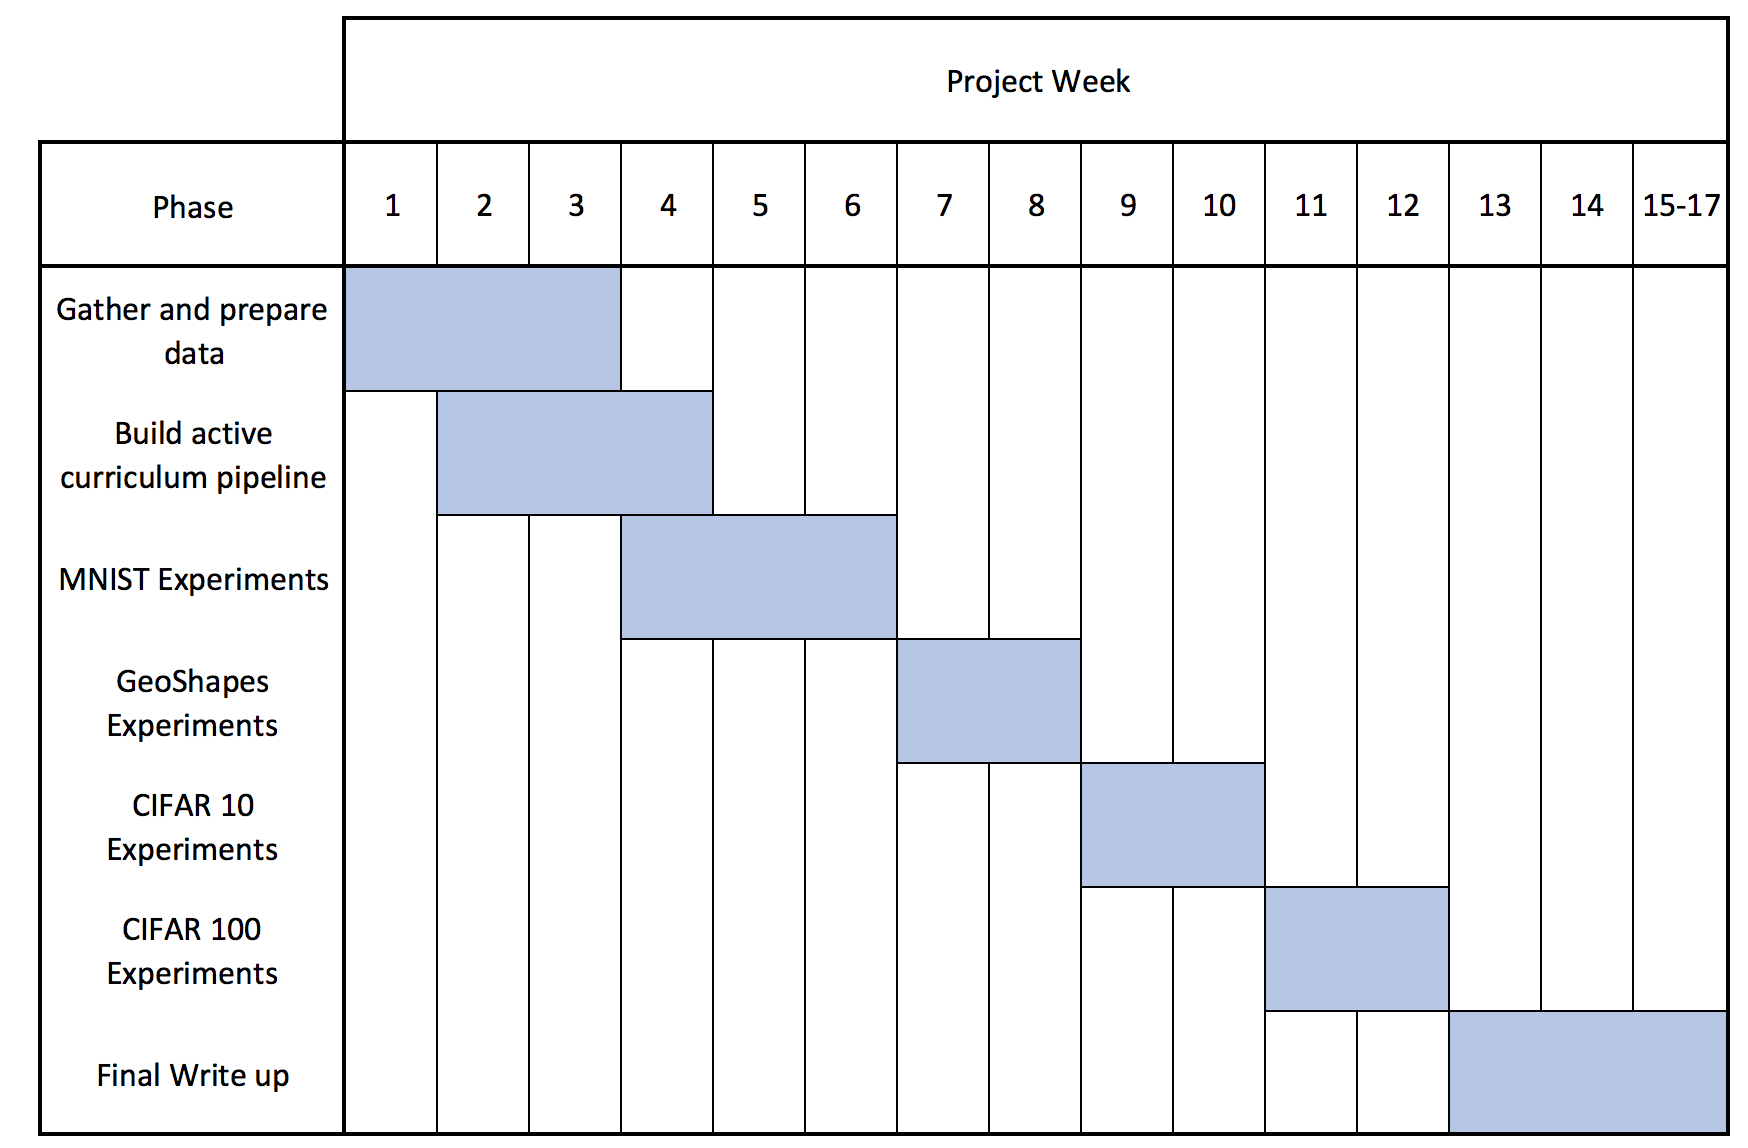
\includegraphics[width=6in]{Timeline_2.png}
\end{center}

\newpage

\begin{thebibliography}{1}
\bibitem{Allgower 1980}
E.L.Allgower and K.Georg, ``Numerical continuation methods. An introduction'', \textit{Springer-Verlag}, 1980
\bibitem{Bengio 09}
Y.Bengio, J.Louradour, R.Collobert and J.Weston, ``Curriculum Learning'', \textit{Procedures of the International Conference on Machine Learning}, 2009
\bibitem{Bubeck 2012}
S.Bubeck, N.Cesa-Bianchi, ``Regret Analysis of stochastic and nonstochastic multi-armed bandit problems'', \textit{Machine Learning}, Issue 5(1), p1-122, 2012
\bibitem{Chang 18}
H-S,Chang, E,Learned-Miller,A.McCallum, ``Active Bias: Training More Accuracy Neural Networks by Emphasizing High Variance Samples'', \textit{Advances in Neural Information Processing Systems 31}, 2018
\bibitem{Cohn 1994}
D.Cohn, L.Atlas and T.Ladner, ``Improving Generalization with Active Learning'', \textit{Machine Learning}, Issue 15, p201-221, 1994
\bibitem{Erhan 09}
D.Erhan, P.A.Manzagol, Y.Bengio, S.Bengio and P.Vincent, ``The difficulty of training deep architectures and the effect of unsupervised pre-training'', \textit{AI \& Statistics}, 2009
\bibitem{Fan 17}
Fan.Yang, Tian.Fei, Qin.Tao, Bian.Jiang, Liu.Tie-Yan, ``Learning What Data to Learn'', \textit{Procedures of the International Conference on Machine Learning}, 2017
\bibitem{Gal 2016}
Y.Gal, R.Islam, Z.Ghahramani, ``Deep Bayesian Active Learning with Image Data'', \textit{Advances in Neural Information Processing Systems, Bayesian Deep Learning workshop}, 2016
\bibitem{Gal 2016 2}
Y.Gal, R.Islam, Z.Ghahramani, ``Dropout as a Bayesian approximation: Representing model uncertainty in deep learning'', \textit{Procedures of the International Conference on Machine Learning}, 2016
\bibitem{Geman 1992}
S.Geman, E.Bienenstock, and R.Doursat, ``Neural networks and the bias/variance dilemma'', \textit{Neural Computation}, Volume 4, p1–58, 1992
\bibitem{Graves 2017}
A.Graves, M.G.Bellemare, J.Menick, R.Munos, and K.Kavukcuoglu. ``Automated curriculum learning for neural networks'', \textit{Proc. Machine Learning Research}, 70, p1311-1320, 2017
\bibitem{Grunwald 2007}
P.D.Gr{\"u}nwald, ``The minimum description length principle'', \textit{The MIT Press}, 2007
\bibitem{Katharopoulos 2018}
A.Katharopoulos and F.Fleuret, ``Not All Samples are Created Equal: Deep Learning with Importance Sampling'', arXiv preprint, arXiv:1803.00942, 2018
\bibitem{Kingma 2015}
D.P.Kingma, T.Salimans and M.Welling, ``Variational dropout and the local reparameterization trick', \textit{Advances in Neural Information Processing Systems 28}, p2575-2583, 2015
\bibitem{Koller 2010}
M.Pawan Kumar, B.Packer, D.Koller, ``Self-Paced Learning for Latent Variable Models'', \textit{Advances in Neural Information Processing Systems 25}, 2010
\bibitem{Own 2000}
A.Owen, Y.Zhou, ``Safe and effective importance sampling'', \textit{Journal of the American Statistical Association}, 95(449), p135-43, 2000
\bibitem{Settles 2009}
B.Settles, ``Active Learning Literature Survey'', Computer Sciences Technical Report 1648, 2009
\bibitem{Weinshall 2018}
D.Weinshall, G.Cohen, ``Curriculum Learning by Transfer Learning: Theory and Experiments with Deep Networks'', arXiv preprint, arXiv:1802.03796, 2018
\end{thebibliography}

\end{document}